
\part{Appendix}






% \section{Vectorization change of basis}
% \label{app:vec-proofs}

% We now prove that the vectorization change of basis operator $T_{\sigma\rightarrow\omega}$ indeed functions as claimed. Let $\2 X$ be a $d$-dimensional complex Hilbert space and let $\{\sigma_\alpha: \alpha=0,...,d^2-1\}, \{\omega_\alpha:\alpha=0,...,d^2-1\}$ be orthonormal operator bases for $L(\2X)$. Define an operator $T_{\sigma\rightarrow\omega}\in \2 L(\XX)$ by
% \begin{equation}
% T_{\sigma\rightarrow\omega}:= \sum_\alpha \ket{\alpha}\dbra{\omega_\omega}_\sigma.
% \end{equation}
% where $\{\ket{\alpha}:\alpha=0,d^2-1\}$ is the computational basis for $\XX$.

% We claim that for any linear operator $A\in L(\2X)$, 
% \begin{equation}
% T_{\sigma\rightarrow\omega}\dket{A}_\sigma=\dket{A}_\omega.
% \end{equation}

% The proof is as follows:
% \begin{eqnarray}
% T_{\sigma\rightarrow\omega}\dket{A}_\sigma
% 	&=& \left(\sum_\alpha \ket{\alpha}\dbra{\omega_\alpha}_\sigma\right)\dket{A}_\sigma\\
% 	&=& \sum_\alpha \ket{\alpha} \dbradket{\omega_\alpha}{A}_\sigma\\
% 	&=& \sum_\alpha \ket{\alpha}\Tr[\omega_\alpha^\dagger A]\\
% 	&=& \dket{A}_\omega.
% \end{eqnarray}


% The inverse of $T_{\sigma\rightarrow\omega}$ is given by
% \begin{equation} 
% T_{\sigma\rightarrow\omega}^{-1}=T_{\sigma\rightarrow\omega}^{\dagger}=T_{\omega\rightarrow\sigma}
% \end{equation}
% and hence $T_{\sigma\rightarrow\omega}$ is unitary.

%%%%%%%%%%%%%%%%%%%%%%%%%%%%%%%%%%%%%%%%%%%%%%%%%%  
\section{Algebra on Quantum States}\label{sec:newalgebra}
We are concerned with a network theory of quantum states.  This on the one hand can
be used as a tool to solve problems about states and operators in quantum theory, but
does have a physical interpretation on the other.  This is not foundational
\textit{per se} but instead largely based on what one 
might call an operational interpretation of quantum states and processes.  A related idea has been used 
to study non-locality in quantum physics \cite{Edwards10}.  This appendix stems from those ideas \cite{Edwards10} which Bill Edwards introduced me to in Oxford around circa 2010.


We call
an algebra a pairing on a vector space, taking two vectors and producing a third
(you might instead call it a monoid if there is a unit, and then a group if the
set of considered vectors is closed under the product).  Let's now examine how every
tripartite quantum state forms an algebra.

Consider a tripartite quantum state (subsystems labeled 1,2 and 3), and then ask the
question: ``how would the state of the third system change after measurement of 
systems one and two?''   Enter Algebras: as stated, an algebra on a vector space, or
on a Hilbert space is formed by a \textit{product} taking two elements from the
vector space to produce a third element in the vector space.  Algebra on states can
then be studied by considering duality of the state, that is considering the
adjunction between the maps of type
\begin{equation}
\I\rightarrow \2 H\otimes \2H \otimes \2H~~~~~~~~\text{and}~~~~~~~~\overline{\2
H}\otimes \overline{\2H} \rightarrow \2H
\end{equation}
This duality is made evident by using the $\dagger$-compact structure of the category
(e.g.\ the cups and caps).  It is given vivid physical meaning by considering the
effect measuring (that is two events) two components of a state has on the third
component.

\begin{remark}[Overbar notation on Spaces] Given a Hilbert space $\2 H$, we can
consider the Hilbert space $\overline{\2H}$ which can be thought of simply as the
Hilbert space $\2 H$ with all basis vectors complex conjugates (overbar).  That is,
$\overline{\2H}$ is a vector space whose elements are in one-to-one
correspondence with the elements of $\2 H$:
\begin{equation}
    \overline{\2H} = \{\overline{v} \mid v \in \2 H\},
\end{equation}
with the following rules for addition and scalar multiplication:
\begin{equation}
    \overline v + \overline{w} =
\overline{\,v+w\,}\quad\text{and}\quad\alpha\,\overline v = \overline{\,\overline
\alpha \,v\,}.
\end{equation}
\end{remark}

\begin{remark}[Definition of Algebra]
We consider an algebra as a vector space $\2A$ endowed with a product, taking a pair
of elements (e.g.\ from $\2A\otimes \2A$) and producing an element in $\2A$.  So the
product is a map $\2A\otimes \2A\rightarrow \2A$, which may not be associative or
have a unit (that is, a multiplicative identity --- see Example \ref{ex:weakunits}
for an
example of an algebra on a quantum state without a unit).
\end{remark}

\begin{observation}[Every tripartite Quantum State Forms an Algebra]
Let $\ket{\psi}\in \2 H\otimes \2H \otimes \2H$ be a quantum state and let
$M_i$, $M_j$ be complete sets of measurement operators.  Then $(\ket{\psi}, M_i,M_j)$
forms
an algebra.
\begin{center}
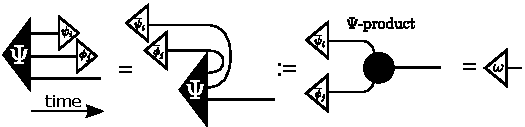
\includegraphics[width=14cm]{algebra-states}
%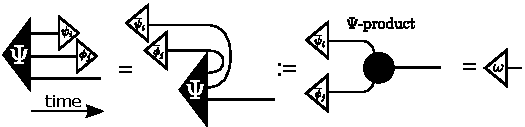
\epsfig{figure=algebra-states,width=14cm}
\end{center}
\end{observation}

The quantum state $\ket{\Psi} = \sum_{ijk}\psi^{ijk}\ket{ijk}$ is drawn as a
triangle, with
the identity operator on each
subsystem acting as time goes to the right on the page (represented as a wire). 
Projective measurements
with respect to $M_i$ and $M_j$ are made.  We define these complete
measurement operators as
\begin{gather}
M_1=\sum_{i=1}^{N}i\ket{\psi_i}\bra{\psi_i}
\end{gather}
\begin{gather}
M_2=\sum_{j=1}^{N}j\ket{\phi_j}\bra{\phi_j}
\end{gather}
such that we recover the identity operator on the $N$-level subsystem viz
\begin{equation}
\sum_{j=1}^{N}\ket{\phi_j}\bra{\phi_j}=\sum_{i=1}^{N}\ket{\psi_i}\bra{\psi_i}=\I_N
\end{equation}
The measurements result in eigenvalues $i,j$ leaving the state of the unmeasured
system in
\begin{equation}
\ket{\omega} = \sum_{xyz}\psi^{xyz} \braket{\overline{\psi}^x}{x}
\braket{\overline{\phi}^y}{y} \ket{z}
\end{equation}
where $\bra{\overline{Q}} \bydef \ket{Q}^\top$ that is, the transpose is factored
into: (i) taking the dagger (diagrammatically this mirrors states across the page)
and (ii) taking the complex conjugate.  Hence,
\begin{equation}
\ket{\overline{Q}}^\dagger = \ket{Q}^\top = \bra{\overline{Q}} =
\overline{\ket{Q}^\dagger}
\end{equation}
and if we pick a real valued basis for $\ket{x},\ket{y},\ket{z}=\ket{0},\ket{1}$ we
recover
\begin{equation}
\ket{\omega} = \sum_{xyz}\psi^{xyz}
\braket{x}{\psi_x}\braket{y}{\phi_y}\ket{z}
\end{equation}

As stated, this physical
interpretation is not our main interest. Even in its absence, we're able to write
down and represent a quantum
state purely in terms of a connected network, where each component is fully defined
in terms of algebraic laws.





\section{\XOR-algebra}\label{sec:Boolean}
Here we review the concept of an algebraic normal form (\ANF) for Boolean
polynomials, commonly known as \PPRM s, (Positive Polarity Reed Muller Forms).  See the reference
book~\cite{Davio78} and the historical references~\cite{Cohn62,
xor70} for further details. 

\begin{definition}
The \XOR{}-algebra forms a commutative ring with presentation
$M=\{\7B,\wedge,\oplus\}$ where the following product is called \XOR
\begin{equation}
\text{---}\oplus\text{---}:\7B\times \7B\mapsto \7B: (a,b)\rightarrow
a+b-ab~\text{mod}~2
\end{equation}
and conjunction is given as
\begin{equation}
\text{---}\wedge\text{---}:\7B\times \7B\mapsto \7B: (a,b)\rightarrow a\cdot b, 
\end{equation}
where $a\cdot b$ is regular multiplication over the reals.  One defines left negation
$\neg(\text{---})$ in terms of $\oplus$ as
$\neg(\text{---})\equiv$
\begin{equation}
  \text{1}\oplus(\text{---}):\7B \mapsto \7B: a\rightarrow 1-a.
\end{equation}
In the \XOR-algebra, 1-5 hold.  (i) $a\oplus 0 = a$, (ii) $a\oplus 1 = \neg a$, (iii)
$a\oplus a = 0$, (iv) $a\oplus \neg a = 1$ and (v) $a\vee b = a\oplus b\oplus
(a\wedge b)$.  Hence, $0$ is the unit of \XOR{} and $1$ is the unit of \AND. The 5th
rule
reduces to $a\vee b = a\oplus b$ whenever $a\wedge b=0$, which is the case for
disjoint ($\text{mod}~2$) sums.  The 
truth table for $\AND$ follows
\begin{center}
% use packages: array
\begin{tabular}{c|c|c}
$~x_1~$ & $~x_2~$ & $f(x_1,x_2)=x_1\wedge x_2$ \\ \hline
0 & 0 & 0 \\
0 & 1 & 0 \\
1 & 0 & 0 \\
1 & 1 & 1
\end{tabular}
\end{center}
\end{definition}

\begin{definition}\label{def:FPRM}
Any Boolean equation may be uniquely expanded to the fixed polarity
Reed-Muller form as:\setlength{\arraycolsep}{0.140em}
\begin{eqnarray}\label{eqn:rm_exp}
&&f(x_1,x_2,...,x_k) = c_0\oplus c_1 x_1^{\sigma_1}\oplus c_2 x_2^{\sigma_2}\oplus
\cdots \oplus c_n x_n^{\sigma_n}\oplus\nonumber\\
&&~~~~~~~~c_{n+1}x_1^{\sigma_1} x_n^{\sigma_{n}}\oplus \cdots \oplus
c_{2k-1}x_1^{\sigma_1} x_2^{\sigma_2},...,x_k^{\sigma_k},
\end{eqnarray}
where selection variable $\sigma_i\in \{0,1\}$, literal
$x_i^{\sigma_i}$ represents a variable or its negation and any $c$
term labeled $c_0$ through $c_j$ is a binary constant $0$ or $1$. In
Equation~\eqref{eqn:rm_exp} only fixed polarity variables appear such that
each is in either un-complemented or complemented form.
\end{definition}

Let us now consider derivation of the form from Definition~\ref{def:FPRM}.  Because
of the structure of
the algebra, without loss of generality, one avoids keeping track of
indices in the $N$ node case, by considering the case where $N\equiv 2^n=8$.

\begin{example}

The vector
\begin{equation}
    \underline{c}=(c_0,c_1,c_2,c_3,c_4,c_5,c_6,c_7,)^\intercal
\end{equation}
represents
all possible outputs of any function $f(x_1,x_2,x_3)$ over the
algebra formed from linear extension of $\7Z_2\times \7Z_2\times \7Z_2$.  We wish to
construct a normal form in terms of the vector $\underline{c}$, where each $c_i\in
\{0,1\}$, and therefore $\underline{c}$ is a selection vector
that simply represents the output of the function
\begin{equation}
    f:\7B\times\7B\times\7B\rightarrow
\7B:(x_1,x_2,x_3)\mapsto f(x_1,x_2,x_3). 
\end{equation}
One may expand $f$ as:
\begin{eqnarray}\label{eqn:generic}
f(x_1,x_2,x_3) &=& (c_0\cdot \neg x_1\cdot \neg x_2\cdot \neg
x_3)\vee(c_1\cdot \neg x_1\cdot \neg x_2\cdot x_3)\vee(c_2\cdot
\neg x_1\cdot x_2\cdot \neg x_3)\nonumber\\
&&\vee(c_3\cdot \neg x_1\cdot x_2\cdot x_3)\vee(c_4\cdot x_1\cdot
\neg x_2\cdot \neg x_3)\vee(c_5\cdot x_1\cdot
\neg x_2\cdot x_3)\nonumber\\
&&\vee(c_6\cdot x_1\cdot x_2\cdot \neg x_3)\vee(c_7\cdot x_1\cdot
x_2\cdot x_3)
\end{eqnarray}

Since each disjunctive term is disjoint the logical \OR{} operation may
be replaced with the logical \XOR{} operation.  By making the substitution $ \neg
a=a\oplus 1$ for all variables and rearranging terms one arrives at
the following normal form:\marginnote{For instance, $\neg x_1\cdot
\neg x_2\cdot\neg x_3=(1\oplus x_1)\cdot(1\oplus x_2)\cdot(1\oplus
x_3)=(1\oplus x_1\oplus x_2\oplus x_2\cdot x_3)\cdot(1\oplus x_3)=
1\oplus x_1\oplus x_2\oplus x_3\oplus x_1\cdot x_3\oplus x_2\cdot
x_3\oplus x_1\cdot x_2\cdot x_3$.}

\begin{eqnarray}\label{eqn:generic2}
f(x_1,x_2,x_3) &=&c_0\oplus(c_0\oplus c_4)\cdot x_1\oplus(c_0\oplus
c_2)\cdot x_2\oplus(c_0\oplus c_1)\cdot x_3\\
&&\oplus(c_0\oplus
c_2\oplus c_4\oplus c_6)\cdot x_1\cdot
x_2\nonumber\\
&& \oplus(c_0\oplus c_1\oplus c_4 \oplus c_5)\cdot x_1\cdot
x_3\oplus(c_0 \oplus c_1 \oplus c_2 \oplus c_3)\cdot x_2\cdot x_3\nonumber\\
&&\oplus (c_0\oplus c_1\oplus c_2\oplus c_3\oplus c_4 \oplus c_5
\oplus c_6\oplus c_7)\cdot x_1\cdot x_2\cdot x_3
\end{eqnarray}

The set of linearly independent vectors, $\{x_1,x_2,x_3,x_1\cdot
x_2,x_1\cdot x_3,x_2\cdot x_3,x_1\cdot x_2\cdot x_3\}$ combined with
a set of scalars from Equation~\ref{eqn:generic2} spans the eight
dimensional space of the Hypercube representing the Algebra.
A similar form holds for arbitrary $N$.

\begin{eqnarray}\label{eqn:generic3}
f(x_1,x_2,x_3) &=& (a_1)\cdot x_1\oplus(a_2)\cdot
x_2\oplus(x_3)\cdot x_3\oplus(a_1\oplus a_2\oplus a_1\oplus
c_2)\cdot x_1\cdot
x_2\nonumber\\
&& \oplus(a_1\oplus a_3\oplus a_1\oplus c_3)\cdot x_1\cdot
x_3\oplus(a_2\oplus a_3\oplus a_2\oplus
c_3)\cdot x_2\cdot x_3\nonumber\\
&&\oplus (a_1\oplus a_2\oplus a_3\oplus a_1\oplus a_2\oplus
a_3)\cdot x_1\cdot x_2\cdot x_3
\end{eqnarray}
\end{example}

\section{The Minimization Method of Karnaugh}\label{appendix:kmap}

The \emph{Karnaugh map} is a tool to facilitate the algebraic reduction of Boolean functions.  Many excellent texts and online tutorials cover the use of Karnaugh maps and should be consulted for more detail.\footnote{This includes the wikipedia entry (\href{http://en.wikipedia.org/wiki/Karnaugh_map}{\tt http://en.wikipedia.org}) and the articles linked to therein as well as the straight forward reference~\cite{Ros99}.}  This Appendix briefly introduces these maps to make the lecture notes self contained.

\begin{comment}
\begin{figure}[t]
\centering
\includegraphics[width=13cm]{kmaps}
\caption{Karnaugh maps: (a) 2-local (positive polarity) variable couplings. (b) Linear (positive polarity) terms.  (c) A Karnaugh map illustrating (with ovals) the linear and quadratic terms needed to an example function.}\label{fig:quad}
\end{figure}
\end{comment}
%%%%%%%%%%%%%%%%%%%%%%%%%%%%%%%%%%%%
%\begin{comment}

\begin{table}
\begin{tabular}{c c c}
\textbf{(a)}\begin{karnaugh-map}[4][2][1][\Large$x_1x_2$][\Large$z_*$] 
\terms{0}{0}
\terms{1}{1}
\terms{2}{2}
\terms{3}{3}
\terms{4}{4}
\terms{5}{5}
\terms{6}{6}
\terms{7}{7}
\implicant{3}{7}
\implicant{5}{7}
\implicant{7}{6}
\end{karnaugh-map}
&\quad
\textbf{(b)}\begin{karnaugh-map}[4][2][1][\Large$x_1x_2$][\Large$z_*$]
\terms{0}{0}
\terms{1}{1}
\terms{2}{2}
\terms{3}{3}
\terms{4}{4}
\terms{5}{5}
\terms{6}{6}
\terms{7}{7}
\implicant{4}{6}
\implicant{1}{7}
\implicant{3}{6}
\end{karnaugh-map}\\
\textbf{(c)}\begin{karnaugh-map}[4][2][1][\Large$x_1x_2$][\Large$z_*$] 
\terms{0}{0}
\terms{1}{0}
\terms{2}{0}
\terms{3}{.}
\terms{4}{.}
\terms{5}{.}
\terms{6}{.}
\terms{7}{0}
\implicant{3}{7}
\implicant{5}{7}
\implicant{7}{6}
\implicant{4}{6}
\end{karnaugh-map}
\end{tabular}
\caption{Karnaugh maps: (a) 2-local (positive polarity) variable couplings. (b) Linear (positive polarity) terms.  (c) A Karnaugh map illustrating (with ovals) the linear and quadratic terms needed to an example function.}\label{fig:quad}
\end{table}

%\end{comment}
%%%%%%%%%%%%%%%%%%%%%%%%%%%%%%%%%%

Karnaugh maps (see Table~\ref{fig:quad} for three examples), or more compactly K-maps, are organized so that the truth table of a given equation, such as a Boolean equation ($f:\mathbb{B}^n\rightarrow \mathbb{B}$) or multi-linear form ($f:\mathbb{B}^n\rightarrow \mathbb{R}$), is arranged in a grid form and between any two adjacent boxes only one domain variable can change value.

This ordering results as the rows and columns are ordered according to Gray code --- a binary numeral system where two successive values differ in only one digit.  For example, the 4-bit Gray code is given as:
\begin{eqnarray*}
&&\{0000, 0001, 0011, 0010, 0110, 0111, 0101, 0100, 1100,\\
&&1101, 1111, 1110, 1010, 1011, 1001, 1000\}.
\end{eqnarray*}
By arranging the truth table of a given function in this way, a K-map can be used to derive a minimized function.

To use a K-map to minimize a Boolean function one \emph{covers} the 1s on the map by rectangular \emph{coverings} containing a number of boxes equal to a power of 2.  For example, one could circle a map of size $2^n$ for any constant function $f=1$.  Table~\ref{fig:quad} (a) and (b) contain three circles each --- all of 2 and 4 boxes respectively. After the 1s are covered, a term in a \emph{sum of products expression}~\cite{Weg87} is produced by finding the variables that do not change throughout the entire covering, and taking a 1 to mean that variable ($x_i$) and a 0 as its negation ($\overline{x_i}$). Doing this for every covering yields a function which \emph{matches} the truth table.

For instance consider Table~\ref{fig:quad} (a) and (b).  Here the boxes contain simply labels representing the decimal value of the corresponding Gray code ordering.  The circling in Table~\ref{fig:quad} (a) would correspond to the truth vector (ordered $z_\star, x_1$ then $x_2$)
\begin{equation}\label{eqn:tt1}
\left(0,0,0,1,0,1,1,1\right)^T.
\end{equation}
The cubes 3 and 7 circled in Table~\ref{fig:quad} correspond to the sum of products term $x_1x_2$.  Likewise (5,7) corresponds to $z_\star x_2$ and finally (7,6) corresponds to $z_\star x_1$. The sum of products representation of (\ref{eqn:tt1}) is simply
\begin{equation*}
f(z_\star,x_1,x_2)=x_1x_2\vee z_\star x_2\vee z_\star x_1.
\end{equation*}
Let us repeat the same procedure for Table~\ref{fig:quad} b.) by again assuming the circled cubes correspond to 1s in the functions truth table.  In this case one finds $z_\star$ for the circling of cubes ladled (4,5,7,6), $x_2$ for (1,3,5,7) and $x_1$ for (3,2,7,6) resulting in the function
\begin{equation*}
f(z_\star,x_1,x_2)=x_1\vee z_\star \vee x_2.
\end{equation*}

\begin{definition}
 (Davio Expansion) The Davio expansion is a decomposition of a boolean function.  
 For a boolean function $f(x_1,...,x_n)$ we set with respect to $x_i$:
    \begin{align} f_{x_i}(x) & = f(x_1,...,x_{i-1},1,x_{i+1},...,x_n) \\[3pt] f_{\overline{x_i}}(x)& = f(x_1,...,x_{i-1},0,x_{i+1},...,x_n) \\[3pt] \frac{\partial f}{\partial x_i} & = f_{x_i}(x) \oplus f_{\overline{x_i}}(x)\, \end{align}
as the positive and negative cofactors of $f$, and the boolean derivation of $f$.  Then we have for the Reed-Muller or positive Davio expansion:
\be
    f = f_{\overline{x_i}} \oplus x_i \frac{\partial f}{\partial x_i}
\ee
\end{definition}



\section{Tensors and Tensor Products}
\label{app:tensor}

The definition of a tensor starts with the \emph{tensor product}~$\otimes$.
There are many equivalent ways to define it, but perhaps the simplest one is
through basis vectors.
Let $V$ and~$W$ be finite-dimensional vector spaces over the same field of scalars~$\K$.
In physics-related applications~$\K$ is typically either the real numbers~$\R$
or the complex numbers~$\C$.
Now $V \otimes W$ is also a vector space over~$\K$.
If $V$ and~$W$ have the bases
$\{e_j\}_j$ and $\{f_k\}_k$, respectively,
the symbols $\{e_j \otimes f_k\}_{jk}$ form a basis for~$V \otimes W$.
Thus, for finite-dimensional spaces
$\dim(V \otimes W) = \dim V \, \dim W$.

The tensor product of two individual vectors $v \in V$ and $w \in W$
is denoted as $v \otimes w$.
For vectors the tensor product is a bilinear map
$V \times W \to V \otimes W$,
i.e.~one that is linear in both input variables.
For finite-dimensional spaces
one can obtain the standard basis coordinates of the tensor product of two vectors
as the \emph{Kronecker product} of the standard basis coordinates of the individual vectors:
\be
(v \otimes w)^{jk} = v^j w^k.
\ee
It is important to notice that due to the bilinearity $\otimes$ maps
many different pairs of vectors~$(v,w)$ to the same product vector:
$v \otimes (s w) = (s v) \otimes w = s (v \otimes w)$, where $s \in \K$.
For inner product spaces (such as the Hilbert spaces encountered in
quantum mechanics) the tensor product space inherits the inner product
from its constituent spaces:
\be
\inprod{v_1 \otimes w_1}{v_2 \otimes w_2}_{V \otimes W} = \inprod{v_1}{v_2}_V \inprod{w_1}{w_2}_W.
\ee
% extended bilinearly...
%$\inprod{T}{S} = T\indices{^{\vec{i}}_{\vec{j}}} S\indices{^{\vec{p}}_{\vec{q}}} g\indices{_{\vec{i}\vec{p}}} g\indices{^{\vec{j}\vec{q}}}$
%where $g\indices{_{\vec{i}\vec{p}}} = \inprod{\bv\spidx{1}{}{i_1}}{\bv\spidx{1}{}{p_1}}\ldots$
%and $g\indices{^{\vec{j}\vec{q}}} = \inprod{\eta\spidx{1}{j_1}{}}{\eta\spidx{1}{q_1}{}}\ldots$

A \emph{tensor}~$T$ is an element of the tensor product of a finite
number of vector spaces over a common field of scalars~$\K$.
%\be
%T \in V_1 \otimes V_2 \otimes \ldots \otimes V_n.
%\ee
The dual space~$V^*$ of a vector space~$V$ is defined as the space of
linear maps from~$V$ to~$\K$. It is not hard to show that $V^*$~is a
vector space over~$\K$ on its own. This leads us to define
the concept of an order-$(p,q)$ tensor, an element of the tensor product
of $p$~primal spaces and $q$~dual spaces:
\be
T \in W_1 \otimes W_2 \otimes \ldots \otimes W_p \otimes V_1^* \otimes V_2^* \otimes \ldots \otimes V_q^*.
\ee
Given a basis $\{\bv\spidx{i}{}{k}\}_k$ for each vector
space~$W_i$ and a dual basis $\{\eta\spidx{i}{k}{}\}_k$ for each dual space~$V_i^*$,
we may expand~T in the tensor products of these basis vectors:
\be
\label{eq:tensorexpansion}
T = T\indices{^{i_1 \ldots i_p}_{j_1 \ldots j_q}}
\bv\spidx{1}{}{i_1} \otimes \ldots \otimes \bv\spidx{p}{}{i_p}
\otimes
\eta\spidx{1}{j_1}{} \otimes \ldots \otimes \eta\spidx{q}{j_q}{}.
\ee
$T\indices{^{i_1 \ldots i_p}_{j_1 \ldots j_q}}$ is simply an array of
scalars containing the basis expansion coefficients.
Here we have introduced the \emph{Einstein summation convention}, in which
any index that is repeated exactly twice in a term, once up, once
down, is summed over. This allows us to save a considerable number of
sum signs, without compromising on the readability of the formulas.
Traditionally basis vectors carry a lower (covariant) index and dual basis vectors
an upper (contravariant) index.

A tensor is said to be \emph{simple} if it can be written as the tensor product
of some elements of the underlying vector spaces:
$T = v\spidx{1}{}{} \otimes \ldots \otimes v\spidx{q}{}{} \otimes \varphi\spidx{1}{}{} \otimes \ldots \otimes \varphi\spidx{p}{}{}$.
This is not true for most tensors; indeed, in addition to the
bilinearity, this is one of the properties that separates tensors from mere Cartesian products of vectors.
However, any tensor can be written as a linear combination of simple tensors,
e.g.~as in Eq.~\eqref{eq:tensorexpansion}.

For every vector space~$W$ there is a unique bilinear map
$W \otimes W^* \to \K$,
$w \otimes \phi \mapsto \phi(w)$
called a natural pairing,
where the dual vector maps the primal vector to a scalar.
One can apply this map to any pair of matching primal and dual spaces in a tensor.
It is called a \emph{contraction} of the corresponding upper and lower indices.
For example, if we happen to have $W_1 = V_1$ we may contract the corresponding indices on~$T$:
\begin{align}
\notag
C_{1,1}(T)
&=
T\indices{^{i_1 \ldots i_p}_{j_1 \ldots j_q}}
\eta\spidx{1}{j_1}{}(\bv\spidx{1}{}{i_1})
\:\:
\bv\spidx{2}{}{i_2} \otimes \ldots \otimes \bv\spidx{p}{}{i_p}
\otimes
\eta\spidx{2}{j_2}{} \otimes \ldots \otimes \eta\spidx{q}{j_q}{}\\
&=
T\indices{^{k \, i_2 \ldots i_p}_{k \, i_2 \ldots j_q}}
\bv\spidx{2}{}{i_2} \otimes \ldots \otimes \bv\spidx{p}{}{i_p}
\otimes
\eta\spidx{2}{j_2}{} \otimes \ldots \otimes \eta\spidx{q}{j_q}{},
\end{align}
since the defining property of a dual basis is
$\eta\spidx{1}{j_1}{}(\bv\spidx{1}{}{i_1}) = \delta\indices{^{j_1}_{i_1}}$.
Hence the contraction eliminates the affected indices ($k$~is summed over),
lowering the tensor order by~$(1,1)$.

We can see that an order-$(1,0)$ tensor is simply a vector,
an order-$(0,1)$ tensor is a dual vector,
and can define an order-$(0,0)$ tensor to correspond to a plain scalar.
But what about general, order-$(p,q)$ tensors?
How should they be understood?
Using contraction, they can be immediately
reinterpreted as multilinear maps from vectors to vectors:
\begin{align}
\label{eq:Tmultilin}
\notag
T':\quad& V_1 \otimes \ldots \otimes V_q \to W_1 \otimes \ldots \otimes W_p,\\
T'(v\spidx{1}{}{} \otimes \ldots \otimes v\spidx{q}{}{}) &=
T\indices{^{i_1 \ldots i_p}_{j_1 \ldots j_q}}
\bv\spidx{1}{}{i_1} \otimes \ldots \otimes \bv\spidx{p}{}{i_p}
\times
\eta\spidx{1}{j_1}{}(v\spidx{1}{}{}) \times \ldots \times \eta\spidx{q}{j_q}{}(v\spidx{q}{}{}),
\end{align}
where we tensor-multiply $T$ and the vectors to be mapped together, and then contract the corresponding indices.
However, this is not the only possible interpretation.
We could just as easily see them as mapping dual vectors to dual vectors:
\begin{align}
\label{eq:Tmultilin2}
\notag
T'':\quad& W^*_1 \otimes \ldots \otimes W^*_p \to V^*_1 \otimes \ldots \otimes V^*_q,\\
T''(\varphi\spidx{1}{}{} \otimes \ldots \otimes \varphi\spidx{p}{}{}) &=
T\indices{^{i_1 \ldots i_p}_{j_1 \ldots j_q}}
\varphi\spidx{1}{}{}(\bv\spidx{1}{}{i_1}) \times \ldots \times \varphi\spidx{p}{}{}(\bv\spidx{p}{}{i_p})
\times
\eta\spidx{1}{j_1}{} \otimes \ldots \otimes \eta\spidx{q}{j_q}{}.
\end{align}
Essentially we may move any of the vector spaces to the
other side of the arrow by taking their dual:
\begin{align}
\label{eq:tensor-interp}
&W \otimes V^*
\quad \isom \quad
\K \to W \otimes V^*
\quad \isom \quad
V \to W
\quad \isom \quad
V \otimes W^* \to \K
\quad \isom \quad
W^* \to V^*,
\end{align}
where all the arrows denote linear maps.
Any and all input vectors are mapped to scalars by the corresponding
dual basis vectors in expansion~\eqref{eq:tensorexpansion}, whereas all input dual vectors map the
corresponding primal basis vectors to scalars.
% TODO We can immediately extend this mapping from simple tensors to general tensors...

If we expand the input vectors~$v\spidx{k}{}{}$ in
Eq.~\eqref{eq:Tmultilin} using the same bases as when expanding the tensor~T,
we obtain the following equation
\begin{comment}
\begin{align}
\notag
T(v\spidx{1}{}{} \otimes \ldots \otimes v\spidx{q}{}{}) &=
T\indices{^{i_1 \ldots i_p}_{j_1 \ldots j_q}}
v\spidx{1}{k_1}{}
\cdots
v\spidx{q}{k_q}{}
\bv\spidx{1}{}{i_1} \otimes \ldots \otimes \bv\spidx{p}{}{i_p}
\times
\eta\spidx{1}{j_1}{}(\bv\spidx{1}{}{k_1}) \times \ldots \times
\eta\spidx{q}{j_q}{}(\bv\spidx{q}{}{k_q})\\
&=
T\indices{^{i_1 \ldots i_p}_{j_1 \ldots j_q}}
v\spidx{1}{j_1}{}
\cdots
v\spidx{q}{j_q}{}
\bv\spidx{1}{}{i_1} \otimes \ldots \otimes \bv\spidx{p}{}{i_p}
\end{align}
where the last step is due to the dual basis definition,
$\eta^i(e_j) = \delta\indices{^i_j}$,
\end{comment}
for the expansion coefficients:
\begin{align}
T'(v\spidx{1}{}{} \otimes \ldots \otimes v\spidx{q}{}{})\indices{^{i_1 \ldots i_p}}
&=
T\indices{^{i_1 \ldots i_p}_{j_1 \ldots j_q}}
v\spidx{1}{j_1}{}
\cdots
v\spidx{q}{j_q}{}.
\end{align}
This is much less cumbersome than Eq.~\eqref{eq:Tmultilin}, and
contains the same information.
This leads us to adopt the \emph{abstract index notation} for tensors,
in which the indices no longer denote the components of the tensor in a
particular basis, but instead signify the tensor's order.
Tensor products are denoted by simply placing the tensor symbols next to each other.
Within each term, any repeated index symbol must appear once up and once down, and denotes
contraction over those indices.
Hence, $x^a$~denotes a vector (with one contravariant index),
$\omega_a$ a dual vector (with one covariant index),
and $T\indices{^{ab}_c}$ an order-$(2,1)$ tensor with two
contravariant and one covariant indices.
$S\indices{^{ab}_{cde}} x^c y^d P\indices{^e_a}$ denotes the contraction of
an order-$(2,3)$ tensor~$S$,
an order-$(1,1)$ tensor~$P$,
and two vectors, $x$ and $y$, resulting in an order-$(1,0)$ tensor
with one uncontracted index,~$b$.


In many applications, for example in differential geometry, the vector spaces
associated with a tensor are often copies of the same vector space~$V$
or its dual~$V^*$,
which means that any pair of upper and lower indices can be contracted,
and leads to the tensor components transforming
in a very specific way under basis changes.
This specific type of a tensor is called an
order-$(p,q)$ tensor \textit{on the vector space}~$V$.
However, here we adopt a more general definition, allowing $\{V_k\}_k$ and
$\{W_k\}_k$ to be all different vector spaces.